\documentclass{article}
\usepackage[utf8]{inputenc}

\title{CS 376 : HW 4 - Continuous Systems}
\author{Fred Eisele }
\date{October 2014}

\usepackage{natbib}
\usepackage{graphicx}
\usepackage{tikz}
\usetikzlibrary{shapes,arrows}

\begin{document}

\maketitle

This problem set is taken from \citep{IntroEmbedSys} chapter 2 : Problem 6.

\section{Problem a}
Using Simulink and its continuous-time modeling component,
see a model of the helicopter control
system shown in \label{fig:control_system}.
Given some reasonable parameters the
actual angular velocity, $\dot{\theta}$, is shown
as a function of time.
The initial and operating conditions
specify that the desired angular velocity
is zero, $\phi (t) = 0$, and that the
top-rotor torque is non-zero,
$T_{top}(t) = b u(t)$ moving to that
value as a step function.
Given are plots for several values of $K_p$.

\begin{figure}[h!]
\centering
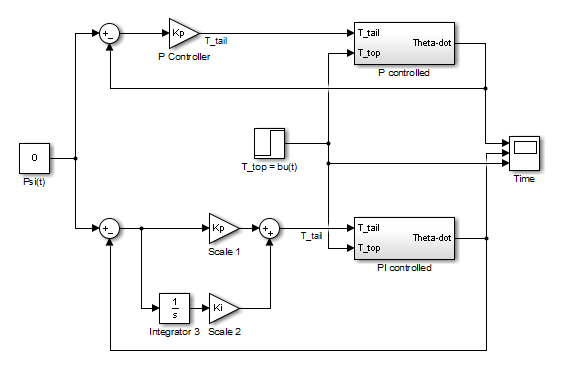
\includegraphics[scale=0.8]{controller_model.png}
\caption{the helicopter models (SimuLink)}
\label{fig:control_system}
\end{figure}

Once the $T_{top}$ has changed a new stable but
typically non-zero $\dot{\theta}$ is approached asymtotically.
Larger values of $K_p$ cause the convergence
to happen more quickly and decrease the value of
the stable $\dot{\theta}$.


\section{Problem b}
Modify the model of part (a) to replace the
\em{P Controller} in the upper portion
of Figure
with the alternative controller shown in the lower
half of Figure.
This alternative controller
is called a proportional-integrator (PI) controller.
It has two parameter $K_p$ and $K_i$.
Experiment with the values of these parameters,
give some plots of the behavior with the
same inputs as in part (a), and discuss the
behavior of this controller in contrast
to the one of part (a).

Once the $T_{top}$ has changed a new (typically non-zero)
$\dot{\theta}$ is approached controlled-variable, $\Psi = 0$,
is approached asymtotically by $\dot{\theta}$
after $T_{top}$ changes.
Larger values of $K_p$ cause the convergence
to happen more quickly.

\bibliographystyle{plain}
\bibliography{references}
\end{document}
